\documentclass{article}
\usepackage{tikz}

\begin{document}

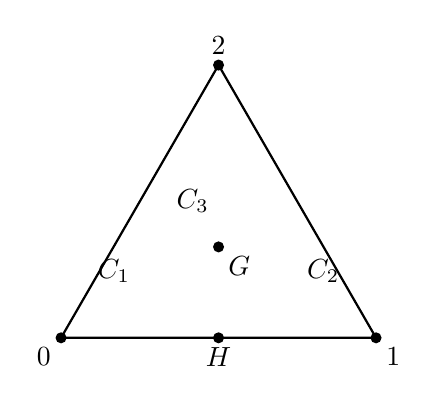
\begin{tikzpicture}[scale=2]
    \draw[thick] (0,0) node[below left] {$0$} -- (2,0) node[below right] {$1$} -- (1,{sqrt(3)}) node[above] {$2$} -- cycle;
    
    % Draw dashed lines
    \draw[dashed] (0,0) -- (2,0);
    \draw[dashed] (0,0) -- (1,{sqrt(3)});
    \draw[dashed] (1,{sqrt(3)}) -- (2,0);

    % Mark points
    \fill (0,0) circle (1pt);
    \fill (2,0) circle (1pt);
    \fill (1,{sqrt(3)}) circle (1pt);
    \fill (1,{sqrt(3)/3}) circle (1pt);
    \fill (1,0) circle (1pt);
    
    % Label points
    \node at (1,{sqrt(3)/3}) [below right] {$G$};
    \node at (1,0) [below] {$H$};
    
    % Draw labels for midpoints
    \node at (0.5,{sqrt(3)/6}) [above left] {$C_1$};
    \node at (1.5,{sqrt(3)/6}) [above right] {$C_2$};
    \node at (1,{sqrt(3)/2}) [left] {$C_3$};
    
\end{tikzpicture}

\end{document}